\documentclass[11pt,a4paper,twoside]{article}
\usepackage[utf8]{inputenc}
\usepackage{polski}



\usepackage{graphicx}
\usepackage{subcaption} % obrazki obok siebie
%\usepackage[caption=false]{subfig} % obrazki nad sobą
\usepackage{wrapfig} 
\usepackage{float}
\usepackage{geometry}
%\geometry{lmargin=3cm,rmargin=2cm, tmargin=2.5cm, bmargin=2.5cm} %marginesy w pracy inż/mgr
\geometry{lmargin=2.5cm,rmargin=2.5cm, tmargin=2.5cm, bmargin=2.5cm} %marginesy ogólne
\usepackage{multirow} % scalanie wierszy tabeli

\usepackage{fancyhdr}
\pagestyle{fancy}
\fancyhead{} % wszystkie nagłówki puste
%\fancyhead[RE,LO]{ Absolwenci Wydziału Prawa  2012}
\fancyfoot{} % wszystkie stopki puste
\fancyfoot[LE,RO]{\thepage}
\renewcommand{\headrulewidth}{0pt}
%\renewcommand{\footrulewidth}{0.4pt}

\usepackage{hyperref}% nazwy odsyłaczy

%unikanie myślników dzielących słowa między liniami
\tolerance=1
\emergencystretch=\maxdimen
\hyphenpenalty=10000
\hbadness=10000

\usepackage{algorithm}
\usepackage{algorithmicx}
\usepackage{algpseudocode}
\makeatletter
\renewcommand{\ALG@name}{Algorytm}
\renewcommand{\figurename}{Wykres}

\usepackage{enumitem}
\setitemize{itemsep=2pt,topsep=2pt,parsep=2pt,partopsep=2pt} %odstępy wyliczanych elementów (-)

\usepackage{indentfirst} % wcięcie w pierwszym akapicie (pod)rozdziału
%%%%%%%%%%%%%%%%%%%%%%%%%%%%%%%%%%%%%%%%% formatowanie kodu R
\usepackage{listings} 
\usepackage{color}
\definecolor{gray}{rgb}{0.5,0.5,0.5}
\lstset{
language=R,
basicstyle=\footnotesize\ttfamily,%\scriptsize\ttfamily,
commentstyle=\ttfamily\color{gray},
numbers=left,
numberstyle=\ttfamily\color{gray}\footnotesize,
stepnumber=0, % numeracja linii
numbersep=5pt,
backgroundcolor=\color{white},
showspaces=false,
showstringspaces=false,
showtabs=false,
frame=none, % obramowanie kodu
tabsize=2,
captionpos=b,
breaklines=true,
breakatwhitespace=false,
title=\lstname,
escapeinside={},
keywordstyle={},
morekeywords={}
}
%%%%%%%%%%%%%%%%%%%%%%%%%%%%%%%%%%%%%%%%%

%%% zawijanie tekstu w tabelach zgodnie z życzeniem
\usepackage{stackengine}
\usepackage{array}
\newcolumntype{L}[1]{>{\raggedright\arraybackslash}p{#1}}
\setstackEOL{\#}
\setstackgap{L}{12pt}
%%%

\usepackage{amsfonts} % zbiory liczba (np. naturalnych)
\usepackage{amsmath} %duże klamry
\usepackage{bbm} %skok jednostkowy
\usepackage[titletoc,title]{appendix} % dodatki - zmiana wyświetlania nagłówka
\pagenumbering{gobble}
\usepackage{afterpage} % pusta strona
\usepackage{tabularx}

%\usepackage{setspace} % interlinia
%\singlespacing 
%\onehalfspacing
%\doublespacing
%\setstretch{0.96}

\begin{document}

\begin{center}
\vspace*{3\baselineskip}
{\LARGE{GIS Projekt}}
\\
\vspace*{1\baselineskip}
{\large{Problem komiwojażera w obecności ulic jednokierunkowych.}}
\\
\vspace*{1\baselineskip}
Tomasz Korzeniowski, 265753\\
Jacek Sochacki, 259741
\\
\vspace*{1\baselineskip}
\today
\end{center}
\section{Zadanie}
Należy zaimplementować (nietrywialny) algorytm rozwiązujący problem komiwojażera, a następnie zbadać, czy można modelować ulice jednokierunkowe w ten sposób, że połączeniu w kierunku A$\rightarrow$B (A, B - wybrane miasta) nadaje się wagę równą odległości miedzy miastami, a połączeniu B$\rightarrow$A nadaje się wagę o bardzo dużej wartości. Głównym celem zadania jest identyfikacja warunków, w których algorytm wskazuje drogę „pod prąd” pomimo istnienia drogi „legalnej”.
\section{Opis zadania}
\subsection{Problem komiwojażera}
Problem komiwojażera można przedstawić następująco. Rozważmy graf $G=(V, E)$, gdzie $V$ to zbiór $n$ miast, które mają zostać odwiedzone przez komiwojażera, natomiast $E$ to zbiór możliwych połączeń między tymi miastami. W ogólności rozważamy graf pełny. Potrzebujemy wyznaczyć macierz kosztów przejść między miastami, czyli wagi krawędzi $c_{ij}$ między miastem $i$ oraz $j$. Do zaznaczenia, którymi krawędziami przejedzie komiwojażer wykorzystamy zmienne binarne $x_{ij}$
$$x_{ij} = 
	\begin{cases} 
      1, & \text{gdy komiwojażer przejeżdża z miasta i do j} \\
      0, & \text{w przeciwnym przypaku}\\
   \end{cases}
$$

Wiadomo, że każde miasto musi być odwiedzone dokładnie raz, z wyjątkiem miasta startowego, w którym komiwojażer zakończy swoją podróż. Sprowadza się to do znalezienia drogi w grafie $G$, której pierwszy i ostatni wierzchołek są tożsame, a koszt przejazdu wyznaczoną drogą jest jak najmniejszy. 

Powyższe zadanie można opisać następującym modelem

\begin{equation}
\min \sum_{i,j \in V} c_{ij} x_{ij} 
\label{f_celu}
\end{equation}
\begin{equation}
\sum_{j \in V} x_{ij}=1, \quad i \in V \backslash \{j\} 
\end{equation}
\begin{equation}
\sum_{i \in V} x_{ij}=1, \quad j \in V \backslash \{i\} 
\end{equation}
\begin{equation}
x_{ij} \in \{0,1\}
\end{equation}
\begin{equation}
x \text{ jest drogą w grafie G}
\end{equation}

%Zauważmy, że model znajduje drogę, a nie cykl. Nie jest to jednak przeszkodą, jeśli założymy, że znalezioną drogę zamkniemy w cykl przez dodanie krawędzi między pierwszym i ostatnim wierzchołkiem.

%Obliczenie kosztu podróży sprowadza się wtedy do wzoru $\sum_{i=1}^{n-1}c_{i(i+1)} + c_{n1}$, gdzie $i$ jest indeksem kolejnego wierzchołka.

Zauważmy, że w macierzy $X = [x_{ij}]_{n\times n}$ w każdej kolumnie i każdym wierszu występuje dokładnie jedna jedynka. Zatem można reprezentować znaleziony cykl jako wektor $w$ kolejnych wierzchołków odwiedzanych przez komiwojażera. Wiemy, że każde miasto występuje w tym wektorze tylko raz, a cykl zamykany jest przez skrajne wierzchołki wektora. Tak utworzony cykl zawsze będzie cyklem Hamiltona, jeśli operacjami wykonywanymi na jego elementach będzie zamiana ich kolejności.

Tak przedstawione zadanie rozwiązuje problem komiwojażera dla grafu pełnego. Zadanie jednak nie jest jedynie problemem komiwojażera. Należy rozważyć połączenia jednokierunkowe między dowolnymi miastami \mbox{$A$ i $B$}, zatem musimy rozważać graf skierowany. Struktura problemu i przyjęty model nie musi być zmieniany. Gwarantuje nam to odpowiednia konstrukcja macierzy kosztów $C = [c_{ij}]_{n\times n}$. W przeciwieństwie do grafu nieskierowanego nie będzie ona symetryczna. Zatem otrzymujemy graf skierowany gdzie ulice jednokierunkowe będą reprezentowane przez krawędzie o nieskończonym koszcie. Ze względu na trudności w implementacji nieskończoności ograniczymy się do dostatecznie dużej wartości takiej krawędzi.

W ramach zadania sprawdzimy czy powyższe modelowanie ulic jednokierunkowych jest wystarczające do znalezienia dopuszczalnego rozwiązania problemu komiwojażera. Spróbujemy wskazać warunki w jakich algorytm znajduje błędne rozwiązania (ulice „pod prąd”).

\subsection{Przeszukiwanie tabu}
Wybranym sposobem rozwiązania problemu będzie algorytm przeszukiwania tabu. Jest to metaheurystyka stosowana do rozwiązywania problemów optymalizacyjnych. Polega na  wykonaniu ciągu kolejnych ruchów w celu przeszukiwania przestrzeni rozwiązań dopuszczalnych zadania. 

Przeszukiwanie tabu rozpoczyna się wybraniem rozwiązania początkowego. W każdej iteracji znajdowane jest rozwiązanie lokalnie najlepsze, a także poszukiwani są sąsiedzi (w zbiorze rozwiązań dopuszczalnych) takiego rozwiązania. Sąsiadem rozwiązania $w$ nazywamy ciąg wierzchołków $w'$, który różni się od oryginalnego na dokładnie dwóch pozycjach. Najlepszy ze wszystkich znalezionych sąsiadów staje się nowym rozwiązaniem lokalnym dla kolejnej iteracji. Najlepszy z sąsiadów charakteryzuje się mniejszą wartością funkcji celu (\ref{f_celu}) od obecnego rozwiązania.

Wybrany algorytm bierze swoją nazwę z ruchów tabu. Jest to sposób zaznaczania, które wierzchołki zostały zamienione. Na listę tabu wpisujemy liczbę iteracji algorytmu, przez którą ponowna zamiana tychże wierzchołków staje się zakazana (tabu). Z każdą iteracją algorytmu czas, przez który wcześniej zazanczony ruch jest zakazany, zostaje zmniejszony o 1. Lista tabu jest listą tylko z nazwy. W rzeczywistości będziemy operowali na macierzy górnej trójkątnej $LT = [lt_{ij}]_{n\times n}$. Element $lt_{ij}$ będzie zawierał informację o liczbie iteracji, przez które zamiana wierzchołków $i$ oraz $j$ jest zakazana. Gdy wartość $lt_{ij} = 0$, dany ruch przestanie być zakazany. 

W implementacji, powyższa dekrementacja listy będzie mało wydajna. Z tego względu będziemy na liście tabu zapisywać aktualny numer iteracji algorytmu powiękoszony o stałą liczbę iteracji przez które dany ruch jest tabu. Do sprawdzenia czy dany ruch jest zakazany, będziemy porównywać wartość listy tabu tego ruchu z akrulnym licznikiem iteracji. Gdy wartość listy tabu będzie co najmniej taka jak aktualy licznik iteracji, ruch przestanie być zakazany. Trudno określić jak długo elementy listy tabu powinny być zakazane. Autorzy \cite{FogelHeurystyka} sugerują by czas pobytu na liście tabu był równy $3n$, gdzie $n$ oznacza liczbę miast problemu.

Na początku działania algorytmu potrzebne jest pewne wstępne rozwiązanie. W naszym przypadku będzie to różnowartościowy ciąg, zawierający wszystkie liczby naturalne ze zbioru $[1,n]$. Rozważamy grafy pełne, więc wybór ulicy jednokierunkowej nie jest przeszkodą. Krawędzie które „nie istnieją” (nie ma połączenia między danymi miastami) lub są to ulice jednokierunkowe mają po prostu bardzo duży koszt.

\subsection{2-opt move}
Poszukiwanie sąsiada $w'$ obecnego rozwiązania wykorzystuje technikę „2-opt move”, Metoda ta została przewidziana dla grafów nieskierowanych. Polega na zamianie dwóch wierzchołków w poszukiwanej drodze, które nie sąsiadują. Zmiana ta powoduje usunięcie dwóch krawędzi z oryginalnej drogi, zamianie wierzchołków i ponowne połączenie przestawionych wierzchołków w drogę. Dla przykładu rozważmy drogę $w$ o następujących wierzchołkach $v$

\bgroup
\def\arraystretch{1.5}
\begin{tabular}{cccccccccccc}
%\hline
Przed zmianą: & $\cdots$ & $v_{i-1}$ & $v_{i}$ & $\mathbf{v_{i+1}}$ & $v_{i+2}$ & $\cdots$ & $v_{j-1}$ & $\mathbf{v_{j}}$ & $v_{j+1}$ & $v_{i+2}$ & $\cdots$\\
Po zmianie: & $\cdots$ & $v_{i-1}$ & $v_{i}$ & $\mathbf{v_{j}}$ & $v_{i+2}$ & $\cdots$ & $v_{j-1}$ & $\mathbf{v_{i+1}}$ & $v_{j+1}$ & $v_{i+2}$ & $\cdots$\\
\end{tabular}
\egroup

Zostały usunięte krawędzie między wierzchołkami $(v_{i}, v_{i+1})$ oraz $(v_{j}, v_{j+1})$, lecz powstały dwie nowe krawędzie $(v_{i}, v_{j})$ oraz $(v_{i+1}, v_{j+1})$. Dla reszty krawędzi pozostała droga przed zmianą, a dla niektórych z nich zmienił się kierunek ich przechodzenia w nowo wyznaczonej drodze. Zamianę tę prezentuje wykres \ref{2opt4krawedzie}a.

Ze względu na skierowanie grafu naszego zadania, technika „2-opt move” zostanie zachowana, lecz zamiast dwóch krawędzi, zostaną zmienione cztery. Wynika to z wykresu \ref{2opt4krawedzie}b. Po dodaniu skierowania cyklu, widać, że nie da się dodać dwóch nowych krawędzi tak, aby pozostałe krawędzie można było przejść zgodnie z ich kierunkiem przed zmianą.

\begin{figure}[ht]
\vspace{-0pt}
\centering
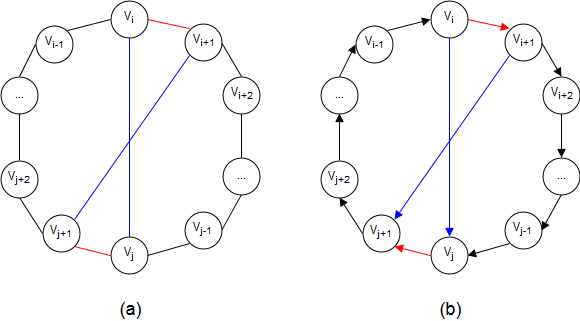
\includegraphics[width=10cm]{2opt4krawedzie}
\caption{Zamiana wierzchołków $v_{i+1}$ oraz $v_{j}$ zgodnie z 2-opt move dla grafu nieskierowanego (a) oraz skierowanego (b).}
\label{2opt4krawedzie}
\end{figure}



Przyjmując zamianę wierzchołków jak w przykładzie grafu nieskierowanego, zostaną usunięte krawędzie $(v_{i}, v_{i+1})$, $(v_{j}, v_{j+1})$ jak poprzednio oraz dodatkowo $(v_{i+1}, v_{i+2})$ i $(v_{j-1}, v_{j})$. Zamiast nich powstaną krawędzie $(v_{i}, v_{j})$, $(v_{i+1}, v_{j+1})$ jak wcześniej oraz nowe $(v_{j}, v_{j+2})$ oraz $(v_{j-1}, v_{i+1})$. Graficznie zamianę tę przedstawia wykres \ref{2optMove}.

\begin{figure}[ht]
\vspace{-0pt}
\centering
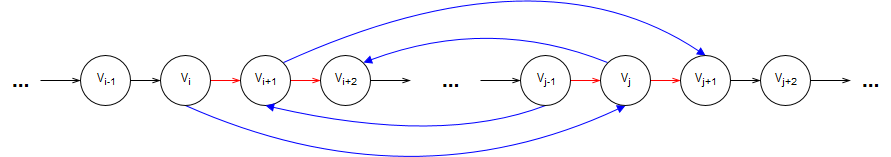
\includegraphics[width=15cm]{2optMove}
\caption{Zamiana wierzchołków $v_{i+1}$ oraz $v_{j}$ zgodnie z 2-opt move dla grafu skierowanego.}
\label{2optMove}
\end{figure}

Taki sposób zamiany niesąsiadujących wierzchołków umożliwia znalezienie wszystkich sąsiadów obecnego rozwiązania. Wystarczy, że sprawdzimy każdą parę wierzchołków, nawet tych sąsiadujących. Sąsiad o najmniejszej wartości funkcji celu stanie się wtedy bieżącym rozwiązaniem. Do obliczenia wartości funkcji celu wystarczy przejść nowo wyznaczonym cyklem, sumując wagi kolejnych krawędzi.

Ponadto, w celu skrócenia czasu wykonania algorytmu wprowadzimy licznik $count$. Będzie on odpowiedzialny za zliczanie iteracji, w których znaleziony sąsiad nie daje lepszego rozwiązania od aktualnie znanego.

\subsection{Kryterium aspiracji}
Może się zdarzyć, że jeden z rozważanych sąsiadów objętych tabu daje świetny wynik, lepszy od jakiegokolwiek rozważanego wcześniej rozwiązania. W standardowym podejściu, algorytm przeszukiwania, wybrałby najlepsze z rozwiązań, w których nie ma ruchów zakazanych. Takie podejście powodowałoby, że algorytm jest mało elastyczny. Jeśli sytuacja jest nietypowa (znaleziono najlepsze ze wszystkich dotąd znanych rozwiązań) możemy zapomnieć o zakazie i wybierzemy nietypowe rozwiązanie. 

\subsection{Schemat algorytmu}
Schemat działania przeszukiwania tabu przestawia algorytm \ref{tabuSearchAlg}. Licznik $tries$ odpowiada za liczbę prób poszukiwania rozwiązania. W ramach każdej próby zostanie wykonanych $iter$ poszukiwań sąsiada i aktualizacji listy tabu. Najlepsze rozwiązanie w danej próbie (lokalne) jest przechowywane w $bestSolverScore$. Jeśli to rozwiązanie jest najlepsze z dotychczas znalezionych dla wszystkich prób (globalne) zostanie zapamiętane w $bestSolutionScore$. Jeśli jednak przez $count$ iteracji algorytmu rozwiązanie nie poprawi się względem dotychczas najlepszego znalezionego, nie ma sensu dalej poszukiwać. Może to wynikać z osiągnięcia minimum lokalnego w przestrzeni rozwiązań dopuszczalnych.

\begin{algorithm}[ht]
\caption{Przeszukiwanie tabu}
\label{tabuSearchAlg}
\begin{algorithmic}%[1]
\Require $C$
	\State $tries$ $\leftarrow$ 0
	\While{$tries$ $\neq$ MAX-TRIES}
		\State wygeneruj drogę początkową $w$
		\State $count$ $\leftarrow$ 0
		\State $iter$ $\leftarrow$ 0
		\While{$iter$ $\neq$ MAX-ITER}
		
		\While{istnieje nieodwiedzony sąsiad $w$} %\Comment{znajdź wszystkich sąsiadów drogi $w$}
		\If{$w'$ ma mniejszą wartość funkcji celu od innych sąsiadów nieobjętych tabu \textbf{LUB} $w'$ spełnia kryterium aspiracji}
		\State zapamiętaj najlepszego sąsiada $w'$
		\EndIf
		\EndWhile
			%\State znajdź wszystkich sąsiadów drogi $w$: $w'$% i wybierz najlepszego z nich: $w'$
			%\State zamień odpowiednie wierzchołki: $w \leftarrow w'$ 
			
			
%			\If{$w$ jest lepsza dla danego $tries$}
%				\State $bestSolverScore \leftarrow w$
%				\State $count$ $\leftarrow$ 0
%				\If{$w$ jest najlepsza dla wszystkich $tries$}
%					\State $bestSolutionScore \leftarrow w$
					
%    			\EndIf
			\State uaktualnij listę tabu: $lt_{ij} \leftarrow iter + 3n$
    		\If{$w'$ jest lepszy od $w$ dla danego $tries$}
    			\State wybierz najlepszego sąsiada: $w \leftarrow w'$ 
				\State $bestSolverScore \leftarrow w$
				\State $count$ $\leftarrow$ 0
				\If{$w$ jest najlepszy dla wszystkich $tries$}
					\State $bestSolutionScore \leftarrow w$
					
    			\EndIf
    		
    		\Else
    			\State ++$count$
    		\EndIf
    		\If{$count =$ MAX-COUNT}
    			\State zbyt długo nie znaleziono lepszego rozwiązania - przerwij tę próbę
    		\EndIf
    	\State ++$iter$
		\EndWhile
		\State ++$tries$
	\EndWhile
\end{algorithmic}
\end{algorithm}



\section{Implementacja algorytmu}

\subsection{Struktury danych}
Do wyznaczenia rozwiązania problemu komiwojażera będziemy potrzebowali
\bgroup
\def\arraystretch{1.5}
\begin{tabularx}{\textwidth}{l|X}
%\hline
$C = [c_{ij}]_{n\times n}$ & Macierz kosztów przejść między $n$ miastami. Zakładamy, że graf jest pełny, a ulice kierunkowe przyjmują wartość wystarczająco dużą, żeby uznać ją za nieskończoność (np. 1e38). Reprezentacją takiej macierzy będzie tablica dwuwymiarowa (tablica tablic) typu zmiennoprzecinkowego podwójnej precyzji (double).\\
$w$ & Wektor reprezentujący drogę komiwojażera. Zawiera indeksy kolejnych odwiedzonych miast, zatem będzie typu całkowitoliczbowego. \\
$LT = [lt_{ij}]_{n\times n}$ & Lista tabu - macierz zakazanych przejść. Element $lt_{ij}$ przechowuje informację o liczbie iteracji przez które zamiana miast $i$ oraz $j$ jest zakazana. Typ całkowitoliczbowy.\\
\end{tabularx}
\egroup

Ponadto będą potrzebne iteratory pętli czy zmienna przechowująca wartość funkcji celu.

\subsection{Projekty testów}
W ramach testów należy sprawdzić poprawność działania algorytmu. Początkowo będzie dany graf pełny, dla którego znany jest koszt drogi optymalnej. Liczba wierzchołków grafu będzie rzędu kilkunastu. Program kilkukrotnie poszuka rozwiązania, a następnie najlepsze z nich zostanie zapamiętane i porównane z rozwiązaniem optymalnym.

Drugim krokiem będzie zakazanie ruchu w określonych połączeniach, które nie należały do najlepszego rozwiązania. Koszt niedozwolonych połączeń będzie zwiększony o umowną wartość nieskończoności - 1e38. Tak dobrana wartość może powodować utratę precyzji, lecz nie jest to problem, gdyż interesuje nas liczba ulic jednokierunkowych w znalezionym rozwiązaniu a nie dokładna wartość funkcji celu rozwiązania. Testy te zostaną poprowadzone dla kilku określonych procentów połączeń jednokierunkowych.
	
Następnie zostaną wygenerowanie losowe macierze kosztów $C$ wraz z zadanym procentem ulic jednokierunkowych. Wagi krawędzi zostaną dostosowane tak, by zapewnić istnienie cyklu Hamiltona w grafie. Pozwoli to zbadać zadania dużej skali (ok. 1000 wierzchołków).
	
Wszystkie te testy zostaną poprowadzone dla różnej liczby miast. Wyniki zostaną przedstawione w postaci tabeli. Dla określonej liczby miast i procentu niedozwolonych połączeń zostanie przedstawiony procent prawidłowych rozwiązań, a dla grafów pełnych podany zostanie również stosunek rozwiązania optymalnego do najlepszego odnalezionego przez algorytm. 
\subsection{Założenia programu}
Implementacja przeszukiwania tabu zostanie wykonana w języku C++. Program będzie wyświetlał na standardowym wyjściu znaleziony cykl komiwojażera oraz jego koszt. Dane o problemie do rozwiązania będą pobierane z pliku tekstowego. W pierwszej linii tego pliku zapisana będzie liczba miast, a w kolejnych koszty przejścia między odpowiednimi nimi, oddzielone spacjami.
%\newpage
  
%\newpage
\begin{thebibliography}{9}
\addcontentsline{toc}{section}{Literatura}
\bibitem{FogelHeurystyka}
Z. Michalewicz, D. B. Fogel
\emph{Jak to rozwiązać czyli nowoczesna heurystyka}.
WNT, Warszawa 2006
\end{thebibliography}
\end{document}